
We have developed a simple simulation tool to evaluate the model
that is publicly available from (URL removed for blind-review).
We omit the details of the simulation settings in this paper but all
the settings are described in the simulation tool.

\subsection{Basic Behaviors}

\begin{figure}[tb]
  \begin{center}
    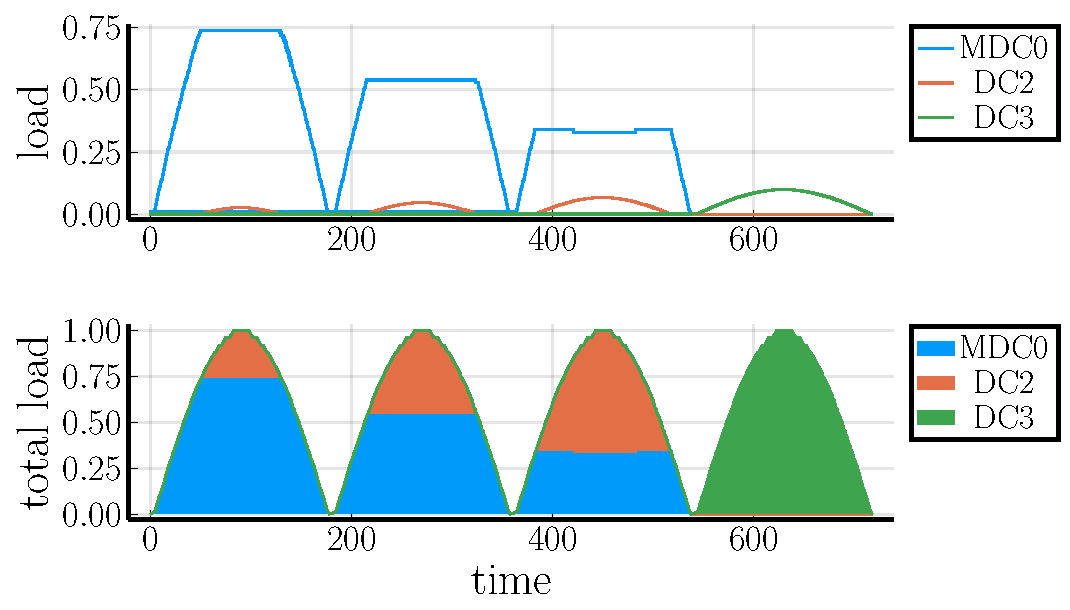
\includegraphics[width=1.0\columnwidth]{fig6-4nodes.pdf}
    \vspace{-2.0ex}
    \caption{Cost manipulations: shifting the load +.2,
      +.4 and raising the weight for data access}
    \smallskip
    \raggedright
    \small
    \Description{Simulation results to illustrate the effects of cost manipulations.}
    \label{fig:lowering}
  \end{center}
\end{figure}

The effects of manipulating the cost function and the resource weight
for a job is illustrated in Figure~\ref{fig:lowering} using the
topology in Figure~\ref{fig:system}.
The capacities of MDC and DC are set to 100 and 1,000.
Note that the capacity of DCs is 10 times larger than that of MDCs
so that DC's load in the top plot looks much smaller for the same
volume of jobs.
In the normalized total load in the bottom plot, the volume is normalized
to the capacity $C$ of MDC to show the total volume of jobs:
$\sum \tilde{\rho}$, \:$\tilde{\rho} = \rho \cdot C/C_{MDC}$.

Here, a series of interactive jobs of the same type are generated in
4 waves between a user at MDC0 and an object at DC3.
In the first wave,  most of the jobs are assigned to the node closest
to the user (MDC0) but some overflowing jobs are offloaded to DC2, the
upstream of MDC0.
The peak load of MDC0 is $.74$ in the first wave.
In the second and the third waves, the cost function of MDC0 is
manipulated to reduce the load by shifting the load by $.2$ and $.4$
respectively. As a result, the peak load of MDC0 is
reduced from $.74$ to $.54$ in the second wave, and then, to $.33$ in the
third wave.
In the fourth wave, the weight for the backend communication is
increased, and all jobs are assigned to the node that has the object
(DC3).

\subsection{Mixed Behaviors}

A more complex scenario is shown in Figure~\ref{fig:mixed}.
Again, the topology in Figure~\ref{fig:system} is used, and
random fluctuation is added to the interval and duration of jobs.
A series of jobs are generated
between user0 at MDC0 and an object at DC3, and
between user1 at MDC1 and an object at DC2.
Both have the ratio of $1:2$ for interactive vs. data-intensive jobs.
To observe offloading behaviors, user1's jobs are increased by a
factor of 2 in the third wave (time 360-540), and by a factor of 10 in
the fourth wave (time 540-720). 
Before time 360, interactive jobs are assigned closer to the users,
and data intensive jobs are assigned closer to the data.
In the third wave, MDC1 reaches the upper limit and overflowing jobs are
assigned to DC2.
In the fourth wave, the link MDC1-DC2 reaches the upper limit so that
overflowing jobs are assigned to DC3.
(To absorb the surge in the fourth wave in this scenario, enough
capacity is provided to the link MDC1-DC3.)
This scenario illustrates the responsive behavior of the system,
and how jobs for MDCs can be offloaded to upstream DCs.

\begin{figure}[tb]
  \begin{center}
    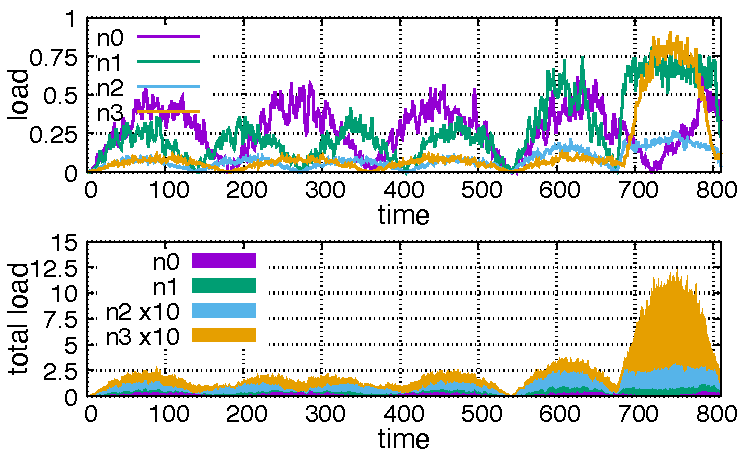
\includegraphics[width=1.0\columnwidth]{simu2.pdf}
    \vspace{-2.0ex}
    \caption{Mixed load with 2 DCs and 2 MDCs}
    \Description{Simulation results with mixed scenario.}
    \label{fig:mixed}
  \end{center}
\end{figure}

% \begin{figure}[tb]
%   \begin{center}
%     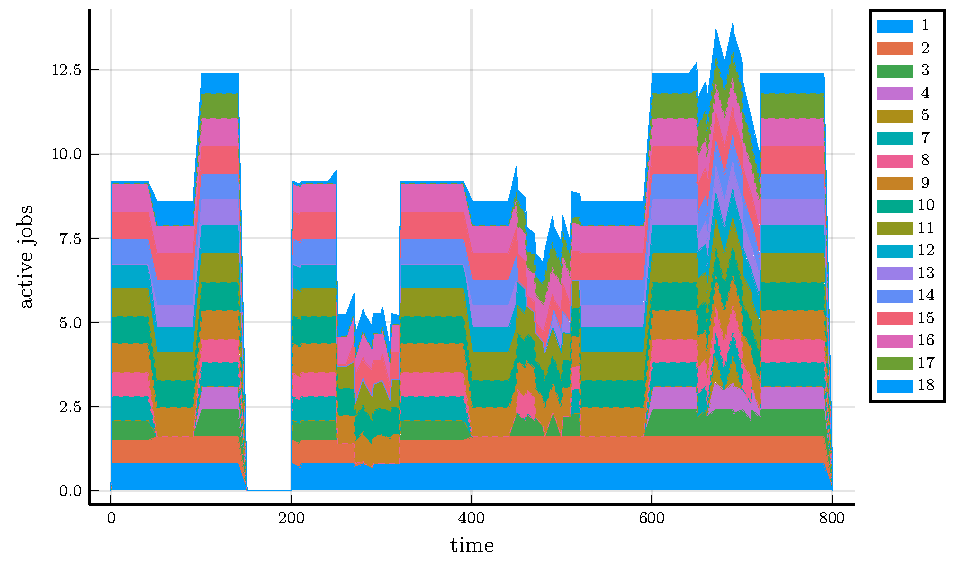
\includegraphics[width=1.0\columnwidth]{complex-convex-monotonic.pdf}
%     \vspace{-2.0ex}
%     \caption{Complex scenario with convex nodes and monotonic links}
%     \label{fig:complex}
%   \end{center}
% \end{figure}

% \begin{figure}[tb]
%   \centering
%   \begin{subfigure}{\columnwidth}
%       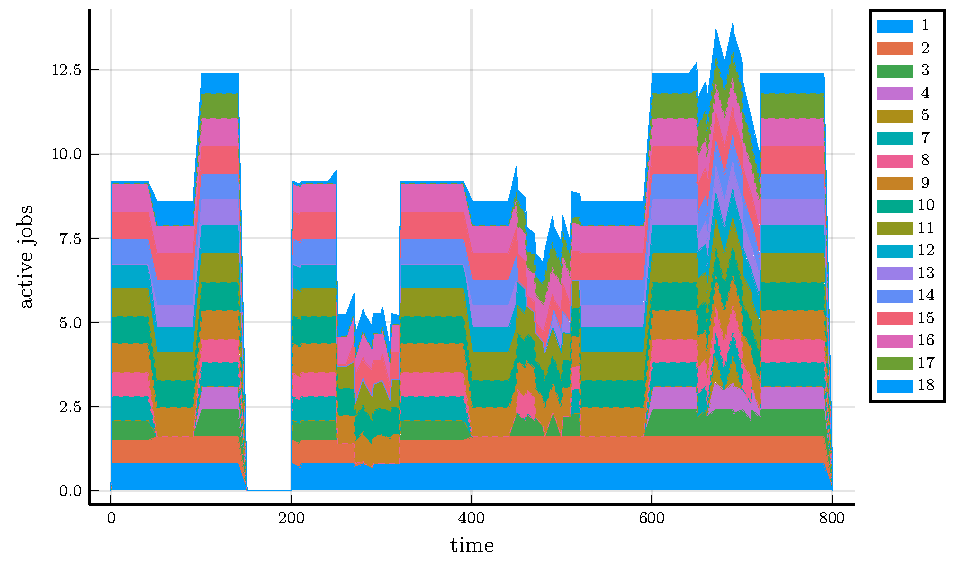
\includegraphics[width=\textwidth]{complex-convex-monotonic.pdf}
%       \caption{Convex nodes and monotonic links}
%       \label{fig:first}
%   \end{subfigure}

%   \begin{subfigure}{\columnwidth}
%       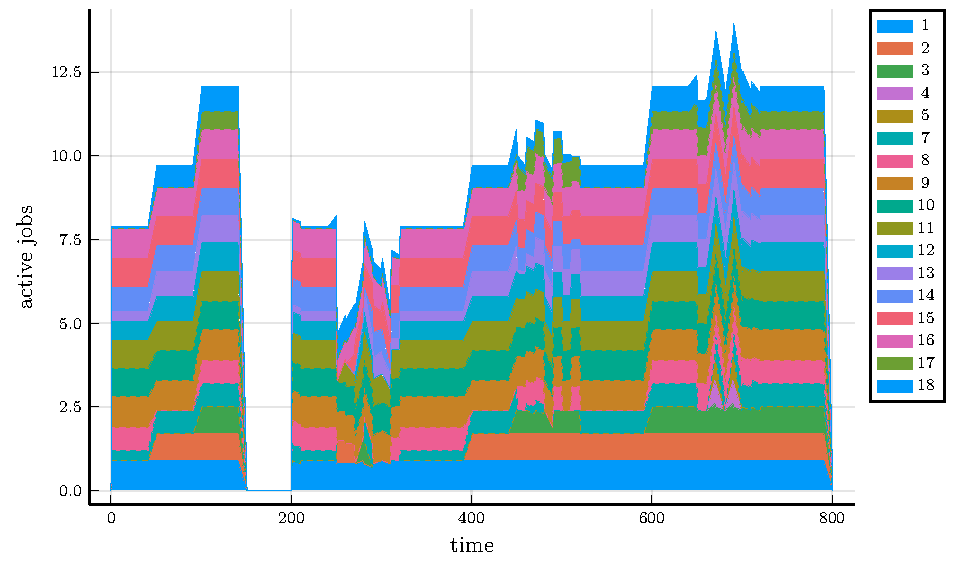
\includegraphics[width=\textwidth]{complex-full-convex.pdf}
%       \caption{Convex nodes and links}
%       \label{fig:second}
%   \end{subfigure}

\begin{figure}[tb]
  \centering
  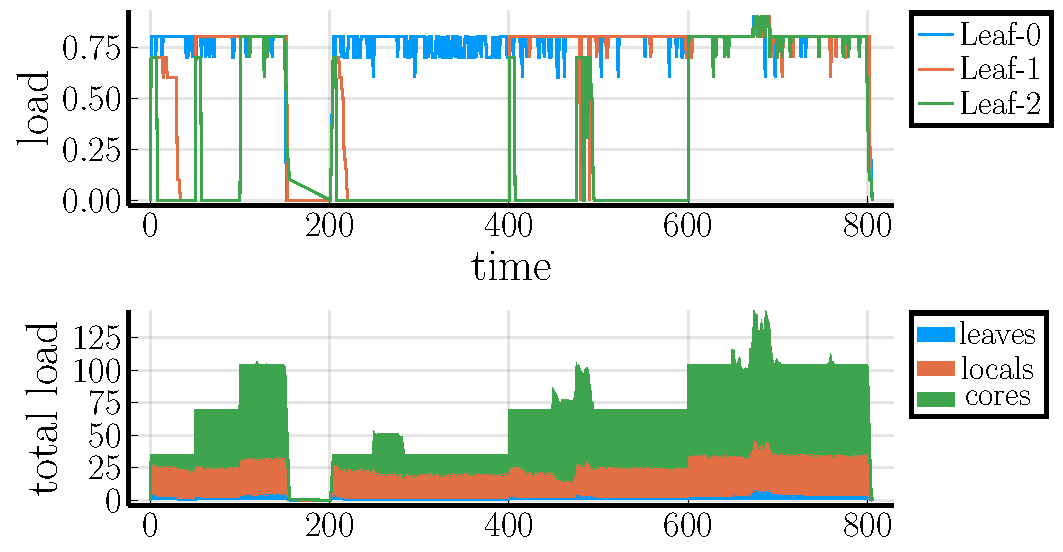
\includegraphics[width=\columnwidth]{18nodes.pdf}
  \vspace{-2.0ex}
  \caption{Mixed load with 18 DCs}
  \Description{A more complex scenario to illustrate offloading behaviors.}
  \label{fig:18nodes}
\end{figure}

The last scenario in Figure~\ref{fig:18nodes} shows a more complex case with
18 DCs: 2 core-DCs (capacity 5,000), 8 local-DCs (capacity 500) and 8 leaf-DCs
(capacity 100) connected by a FAT-tree.
Each leaf-DC is connected to one local-DC, and each local-DCs is connected to
2 other local-DCs; 4 of the local-DCs are also connected to 2 core-DCs.
The bottom plot shows the normalized total load $\sum \tilde{\rho}$
divided into the 3 DC classes.
Jobs are generated from 3 leaf-DCs at 3 levels with additional surges,
and data objects are randomly populated at all leaf-DCs and local-DCs.
The bottom plot shows how excess jobs are offloaded to upstream DCs,
and the top plot shows the loads of the 3 job-generating leaf-DCs.
Although the leaf-DCs handle only a small fraction of the total jobs,
the loads of the leaf-DCs stay at around $.75$ while they are
active, except a short transient overshoot during the surge from time
680.

Overall, the simulation results illustrate quick responses to changing
load by offloading excess jobs to upstreams,
yet converging to stable states once the load is settled,
while maintaining the load for each active resource at around the target
range.

